\chapter{System Design}

This chapter presents the overall architecture and design of the system. This chapter introduces and explains the various design 
paradigms used for the development and deployment of various components that interact together to provide the functionalities of the system. 

The system architecture calls for a relational database to store aggregated users test and biometric data, a RESTful API to provide secured 
and customized access to user data in the database, and a web application to provide a user interface for administrative access to the 
system. Machine learning services were developed and deployed to provide real-time machine learning data analysis and best model selection 
algorithms.

The various components interact together to provide the system functionalities and were developed and deployed in a loosely coupled manner and
interact with each other through well defined RESTful API calls.  The Amazon Web Services (AWS) cloud platform was utilized as a Infrastructure
as a Service (IaaS) to provide the compute and storage resources required to run the various components with the EC2 Micro Virtual Machine, 
domain name service was provided using Amazon Route 53 (Domain Naming Service) and Amazon Certificate Manager for TSL/SSL security. Relational 
Database was provided as a microservice using the Amazon Relational Database Service (MySQL)

\begin{figure}[h!]
    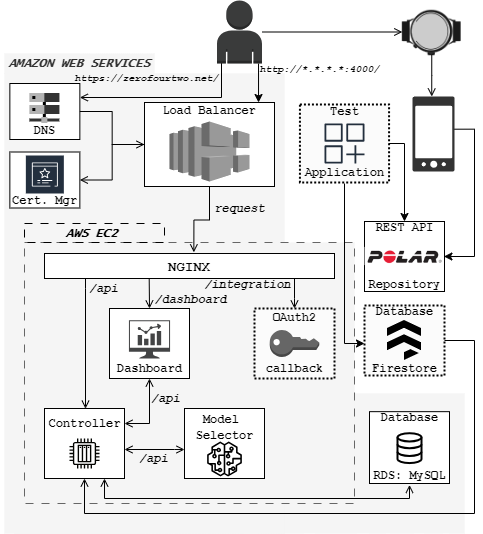
\includegraphics[width=0.9\textwidth]{images/sys_architecture.png}
    \caption{System Architecture.}
    \label{image:sys_architecture}
\end{figure}

\section{System Architecture}

The Overall system was designed for a public cloud deployment while the core functionalities of the system was modelled using the
Model-View-Controller (MVC) Software Architectural Pattern. Thus, the system was divided into three major components: the Model, comprising 
of the databases and the machine learning models; the View, implemented with Dashboard web application; and the Controller, implemented with 
the Controller web application. Each of these components were developed and deployed as separate services. 

\begin{figure}[h!]
    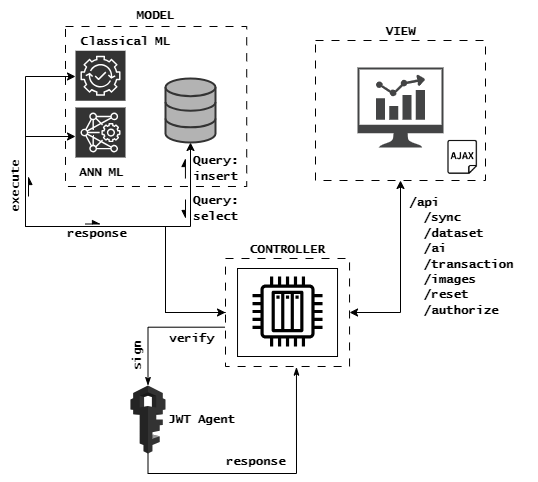
\includegraphics[width=0.9\textwidth]{images/mvc_arch.png}
    \caption{MVC Architecture.}
    \label{image:mvc_arch}
\end{figure}

\section{Routing \& Security}
Communication between various components was modelled with the client-server paradigm utilizing REST API over HTTP. Communication may be initiated
by a client and information exchanged with a server using a request-response messaging pattern.  
Security was provided to secure access to the system and data. At the network level, the TSL/SSL security layer was added to the domain name to 
provide end-to-end encryption between the user and the web application. At the application api level, the Bearer Authentication Token was used to 
secure access to the REST API. Figure~\ref{image:comm_sec} shows a detailed address resolution, traffic routing, security validation and 
request-response path between a client and the web application. 

\begin{figure}[h!]
    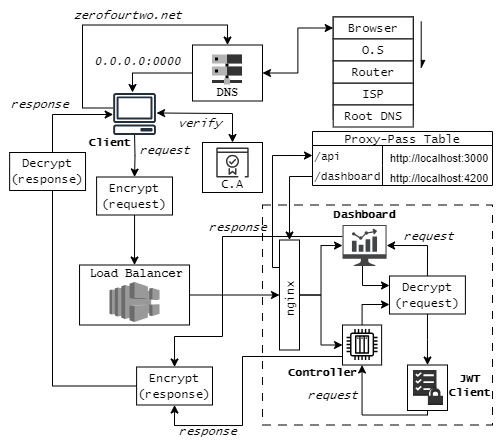
\includegraphics[width=0.9\textwidth]{images/comm_sec.png}
    \caption{Communication \& Security.}
    \label{image:comm_sec}
\end{figure}

\subsubsection*{Domain Name} A domain name was registered on Route 53 and linked to the Elastic Load Balancer (ELB) to provide a consistent means of 
accessing the web application. Assigned IP addresses to an instance of the EC2 Micro Virtual Machine are not static and will change each time the 
instance is restarted, this is guaranteed to break connection to the application. Situations like this are undesirable, and requires frequent 
modification of configuration files every time the IP address changes. Figure~\ref{image:dns_record} shows the domain name configuration on Route 53.

\begin{figure}[h!]
    \begin{center}
        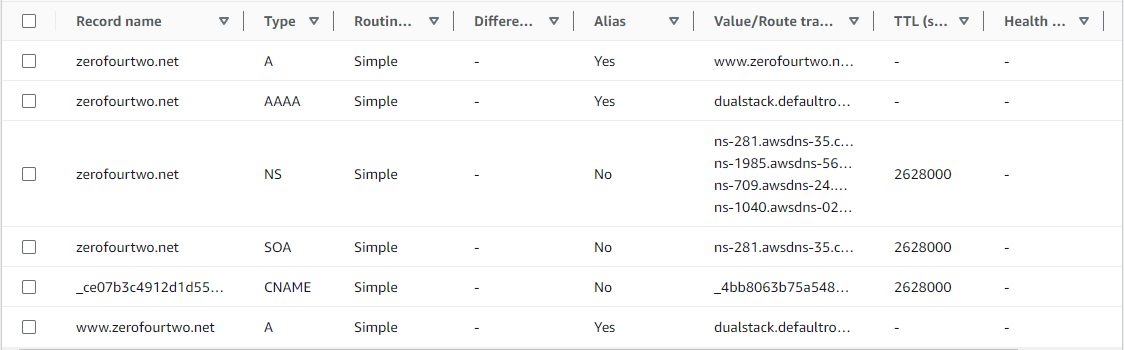
\includegraphics[width=0.9\textwidth]{images/dns_record.png}
        \caption{DNS Records}
        \label{image:dns_record}
    \end{center}
\end{figure}

\subsection{REST API}
The Representational State Transfer (REST) API standard was used to provide a stateless communication between various components of the system. 
The JSON data format was used to represent the data exchanged between the components. Functionalities of the web application is accessed using a 
client browser and thus requires a front end application to interact with the user. The front end application referred to as the Dashboard was
designed and deployed as a stand alone application and requires data from the Models to perform its functionalities. A REST API was designed and 
developed to provide customized access to the data in the Models. 
Table~\ref{table:rest_api} shows the list of the various endpoints of the API. 

\begin{table}
    \centering
    \resizebox{\textwidth}{!}{
    \begin{tblr}{|l|l|l|l|l|l|l|}
    \hline
    \textbf{Endpoint} & \textbf{Auth.} & \textbf{Params.} & \textbf{Query} & \textbf{Body}    & \textbf{Desc.} & \textbf{Resp.} \\
    \hline
    GET /api/dataset & Bearer           & -                  & columns        & -                & Get dataset          & 200 \\
    GET /api/sync    & Bearer           & -                  &                & -                & Sync database        & 200 \\
    GET /api/reset   & Bearer           & -                  & -              & -                & Reset database       & 200 \\
    GET /api/ai           & Bearer           & /:id               & -              & -                & Run M/L with id      & 200 \\
    GET /api/transactions & -                & /:id               & -              & -                & Get results for id   & 203, 200 \\
    GET /api/images       & -                & /:id/path          & -              & -                & Get image            & 200 \\
    POST /api/authorize     & Bearer           & -                  & -              & json             & Authorize user       & 200 \\
    \hline    
\end{tblr}}
    \caption{REST API Endpoints}
    \label{table:rest_api}
    \end{table}


\subsection{Security}
The AWS Certificate Manager was used to provide the TSL/SSL security layer to the domain name, and handles all the complexity involved in 
key management and certificate provisioning \cite{aws_acm}. Incoming request is routed to the LoadBalancer which was configured to re-route all incoming traffic 
to a registered target which is the EC2 Virtual Machine instance. The TSL/SSL security layer was attached to the LoadBalancer as a security policy 
to provide end-to-end encryption. The value for the domain name $A$ and $AAAA$ records were set to the LoadBalancer DNS name, while the value 
for the domain name $CNAME$ record was set to that the certificate provided by the AWS Certificate Manager. 
Figure~\ref{image:ssl_record} shows the TSL/SSL record configuration on Certificate Manager. 

\begin{figure}[h!]
    \begin{center}
        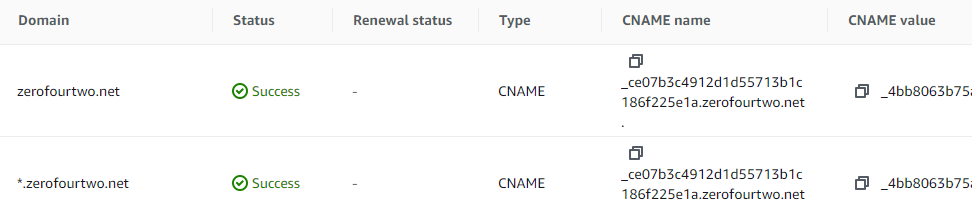
\includegraphics[width=0.9\textwidth]{images/ssl_record.png}
        \caption{TSL/SSL Record}
        \label{image:ssl_record}
    \end{center}
\end{figure}

The Bearer Authentication Token was used to further secure access to specific endpoints of the REST API. Consumers of the API are required to 
provide a valid token as a header in a request to successfully access the API. Generating a token involves digitally signing user information 
comprising of the header, payload and signature; using a secret key only known to the server. Decoding the token involves verifying the signature 
using the secret key to ensure the token is valid, then user information is extracted from the payload. Figure~\ref{image:jwt} illustrates the 
process of signing and verifying a JWT. 

\begin{figure}[h!]
    \begin{center}
        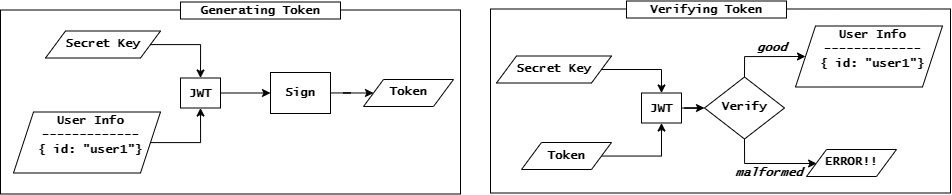
\includegraphics[width=0.9\textwidth]{images/jwt.png}
        \caption{JWT Token}
        \label{image:jwt}
    \end{center}
\end{figure}


\section{Controller}
In a Model-View-Controller (MVC) architectural pattern, the Controller is at the center of the system's process flow and is responsible for 
handling user requests and producing an appropriate response to requests. The Controller was developed as a standalone web application
listening on port 3000 and is capable of servicing multiple requests concurrently and referentially coupled with the Model. The Controller
provides an interface for users to interact with the Models using RESTful API calls. Figure~\ref{image:uml_controller} shows the UML diagram of the 
Controller implementation.
\begin{figure}[h!]
    \begin{center}
        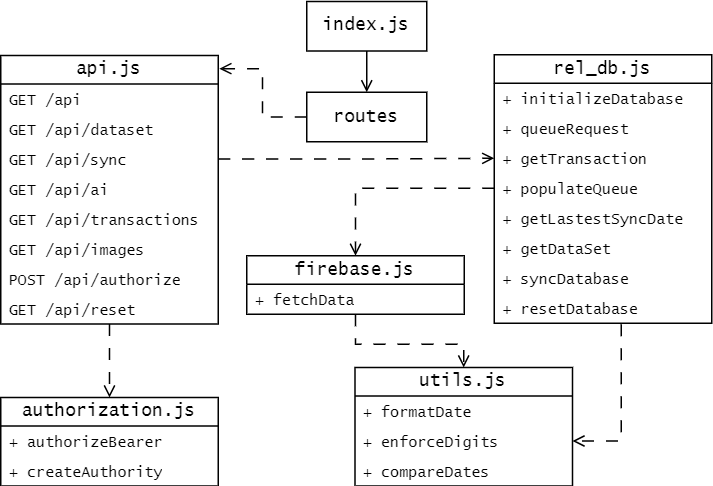
\includegraphics[width=0.7\textwidth]{images/uml_controller.png}
        \caption{Controller UML Diagram.}
        \label{image:uml_controller}
    \end{center}
\end{figure}

\section{View}
The View component of the system otherwise known as the Dashboard was implemented as a standalone web application running on port 4200. The 
Dashboard provides an interface for users to interact with the system and consume the functionalities and data provided by the Controller
Models respectively. The Dashboard provides both administrative and data analysis functionalities. The administrative functionalities include
pulling user data from the Firestore database, synchronizing the relational database with the Firestore database, resetting the relational 
database, setting up user authentication. The data analysis functionalities include filtering data for analysis and running machine learning
algorithms for performance prediction. The Dashboard also allow users to visualize the results from the machine learning algorithms. 

To provide real-time information to the user, the Dashboard utilizes Asynchronous Javascript and XML (AJAX) to make asynchronous requests to
the controller and lazily updates the user interface with eventual response from the controller. 

\section{Model}
The Model component of the system comprises the Machine Learning Models and the Databases. The controller queries the Models and gets a 
response which is passed on to the View on request.

\subsection{M/L Models}
For the purpose of finding correlation and predicting user performance given their biometric data, two different Machine Learning models 
were designed and developed. The models were designed to predict user's performance based on their biometric data. 
Algorithm and hyperparameter tuning was performed to select the best model for the Automatic Neural Network and Classical M/L Algorithms.
An adhoc messaging protocol was developed to interact with the models and provide a comprehensive feedback about model performance. 
The M/L Algorithms were deployed as standalone services that can be activated by the Controller on request. On the low level, the Controller
fires up the M/L Algorithm service and passing in a session identification parameter which is a unique identifier to a path where output from the
M/L Algorithm is stored. Response from the M/L Algorithm is then read by the Controller and stored in the database. Further down the pipeline
any enquiry for the stored session will be used to identify and retrieve associated resource from the database. Fig.~\ref{image:model_comm}
shows the sequence of interactions between the Controller and the M/L Algorithm.

\begin{figure}[h!]
    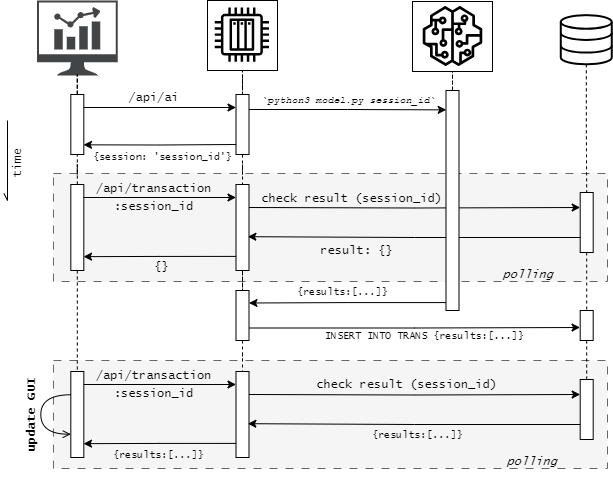
\includegraphics[width=0.9\textwidth]{images/model_comm.png}
    \caption{M/L Model Communication.}
    \label{image:model_comm}
\end{figure}

\subsubsection{Classical M/L Algorithm} 
The model selection algorithm was developed to compare various classical machine learning algorithms and select the best performing model. For
every independent variable, the algorithm compares the performance of the various models using a 5-fold cross validation technique and selects
the best model. Machine learning algorithms used in the model selection include: Linear Regression, Support Vector Machine, Random Forest and 
K-Nearest Neighbors. 

\subsubsection{Automatic Neural Network}

A fully-connected Automatic Neural Network was developed to solve the same problem and provide a different perspective to the problem. The
rationale for developing the Automatic Neural Network was to provide a more complex model capable of learning more complex pattern in the data.


\subsection{Databases}
The database stores user's information and provide a convenient and efficient way of accessing user's data. The relational database provides all
data required to run the application and the firebase database provides an unstructured data bank for user's information from where data is sourced
for further regularization. 
\subsubsection{Relational Database}
The relational database was designed to store user's information and other information required to effectively manipulate, update, store and view 
the application state. Figure~\ref{image:db_schema} shows the database schema. 
\begin{figure}[h!]
    \centering
    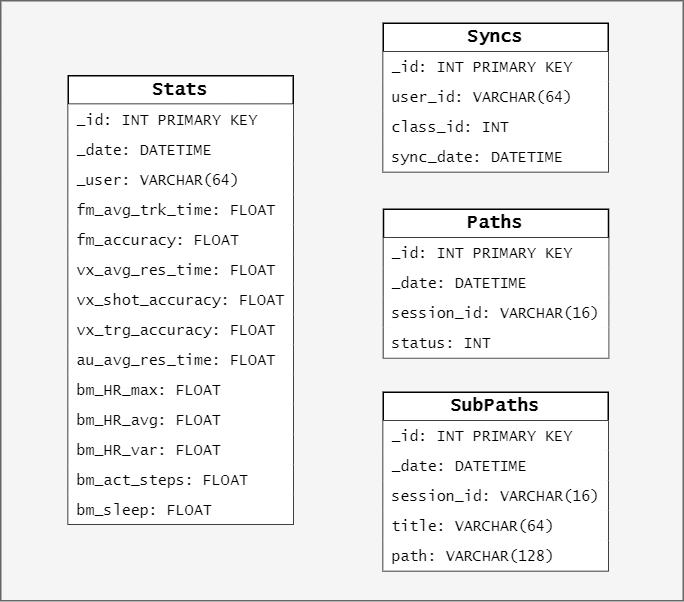
\includegraphics[width=0.7\textwidth]{images/db_schema.png}
    \caption{Database Schema}
    \label{image:db_schema}
\end{figure}
\subsubsection{Firestore Database}
The Firebase database is part of the inherited infrastructure for this project. Data collected from the Polar Vantage V2 smartwatch and the Test 
Application are stored as documents in separate collections. These unstructured data requires further processing collation before use, thus they 
are aggregated and synchronized with the relational database. Figure~\ref{image:db_sync} shows the process of synchronizing the Firestore database
with the relational database.
\begin{figure}[h!]
    \centering
    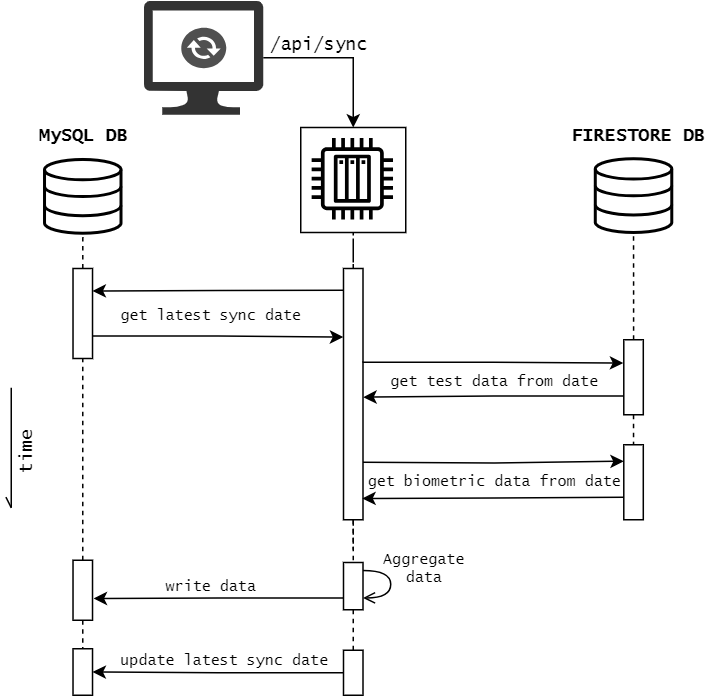
\includegraphics[width=0.7\textwidth]{images/db_sync.png}
    \caption{Database Synchronizing}
    \label{image:db_sync}
\end{figure}



The machine learning services were developed using the 
sklearn library, Keras TensorFlow library and Flask web framework. The services were deployed on a cloud server to provide real-time best
model selection for users' performance prediction.

\section{Inherited Infrastructure}

A desktop application Test Platform was part of the inherited infrastructure for this project and was used to generate test data.
The Test Platform was developed using Unity3D Game Engine and C\# programming language. Results from the Test Platform were stored in 
a Firestore database. The Firestore database which is a document based database, and provides a convenient and efficient storage for 
unstructured data as obtainable in the Test Platform. The database also provides a very secured and scalable storage solution with 
real-time access.

For the purpose of collecting biometric data, the Polar Vantage V2 smartwatch was used. The smartwatch manufacturer provides a RESTful API
repository for storing and accessing user's data collected by the smartwatch. The TestPlatform application provides functionalities to 
access the API and retrieve relevant biometric data from the smartwatch. The data is then stored in the Firestore database.

User authentication endpoint for Auth2.0 flow required for enrolling volunteers into the system was also inherited from the previous project. 
The endpoint was developed using Express.js and Embedded Javascript (EJS) technologies. The endpoint provides a secure way to authenticate
users on the Polar Flow API to grant access to the users' biometric data. 